\chapter{Testy aplikacji backendowej}

\section{Testy jednostkowe}
Testowanie aplikacji backendowej jest kluczowym elementem zapewniającym jakość i stabilność oprogramowania. W tym rozdziale przedstawiono strukturę testów jednostkowych zaimplementowanych w projecie z wykorzystaniem frameworków Spring Boot oraz JUnit 5. Testy podzielono na różne moduły, takie jak blockchain, kryptowaluty, NFT, oraz zasoby. Pozwoliło to na łatwiejsze zarządzanie i rozwój aplikacji. Testy integracyjne i wydajnościowe zostaną przeprowadzone w przyszłości.

\subsection{Testy w module Blockchain}

Moduł blockchain zawiera testy związane z obsługą różnych łańcuchów bloków, takich jak Bitcoin, Ethereum i Solana. Poniżej przedstawiano przykłady testów dla różnych podkategorii.

\subsubsection{Testy dla Bitcoin}

Przykładowy test dla klasy \texttt{BitcoinAccountControllerTest}

\begin{lstlisting}[language=Java, style=JavaStyle]
package org.example.backend.blockchain.bitcoin.accounts.controller;
import ...

class BitcoinAccountControllerTest {
    @Mock
    private BitcoinAccountService bitcoinAccountService;

    @InjectMocks
    private BitcoinAccountController bitcoinAccountController;

    @BeforeEach
    void setUp() {
        MockitoAnnotations.openMocks(this);
    }

    @Test
    void testGetAccountData_Found() {
        String address = "testAddress";
        BitcoinAccountDto bitcoinAccountDto = new BitcoinAccountDto();
        when(bitcoinAccountService.getAllAccountData(address)).thenReturn(bitcoinAccountDto);
        ResponseEntity<BitcoinAccountDto> response = bitcoinAccountController.getAccountData(address);
        assertEquals(ResponseEntity.ok(bitcoinAccountDto), response);
        verify(bitcoinAccountService, times(1)).getAllAccountData(address);
    }

    @Test
    void testGetAccountData_NotFound() {
        String address = "testAddress";
        when(bitcoinAccountService.getAllAccountData(address)).thenReturn(null);
        ResponseEntity<BitcoinAccountDto> response = bitcoinAccountController.getAccountData(address);
        assertEquals(ResponseEntity.notFound().build(), response);
        verify(bitcoinAccountService, times(1)).getAllAccountData(address);
    }
}
\end{lstlisting}

\subsubsection{Testy dla Ethereum}
Przykładowy test dla klasy \texttt{EthereumAccountControllerTest}

\begin{lstlisting}[language=Java, style=JavaStyle]
package org.example.backend.blockchain.ethereum.accounts.controller;
import ...

class EthereumAccountControllerTest {
    @Mock
    private EthereumAccountService ethereumAccountService;

    @InjectMocks
    private EthereumAccountController ethereumAccountController;

    @BeforeEach
    void setUp() {
        MockitoAnnotations.openMocks(this);
    }

    @Test
    void getEtherBalanceAndTransactionHistory() {
        EthereumAccountDto ethereumAccountDto = new EthereumAccountDto();
        when(ethereumAccountService.getEtherBalanceAndTransactionHistory(anyString())).thenReturn(Optional.of(ethereumAccountDto));
        Optional<EthereumAccountDto> result = ethereumAccountController.GetEtherBalanceAndTransactionHistory("testAddress");
        assertTrue(result.isPresent());
        assertEquals(ethereumAccountDto, result.get());
    }

    @Test
    void getTokenBalance() {
        when(ethereumAccountService.getTokenBalance(anyString(), anyString())).thenReturn(100.0);
        ResponseEntity<Double> response = ethereumAccountController.getTokenBalance("testAddress", "testContractAddress");
        assertEquals(200, response.getStatusCodeValue());
        assertEquals(100.0, response.getBody());
    }
    ...
}
\end{lstlisting}

\subsubsection{Testy dla Solana}

Przykładowy test dla klasy \texttt{SolanaAccountControllerTest}

\begin{lstlisting}[language=Java, style=JavaStyle]
package org.example.backend.blockchain.solana.accounts.controller;
import ...

public class SolanaAccountControllerTest {
    @Mock
    private SolanaAccountService solanaAccountService;

    @InjectMocks
    private SolanaAccountController solanaAccountController;

    @BeforeEach
    public void setUp() {
        MockitoAnnotations.openMocks(this);
    }

    @Test
    public void testGetSolanaAccountBalance() {
        String address = "someAddress";
        String balance = "1000";
        when(solanaAccountService.getAccountBalance(address)).thenReturn(Optional.of(balance));
        ResponseEntity<String> response = solanaAccountController.getSolanaAccountBalance(address);
        assertNotNull(response);
        assertEquals(HttpStatus.OK, response.getStatusCode());
        assertEquals(balance, response.getBody());
    }
    ...
}
\end{lstlisting}

Pozostałe klasy przetestowano podobnie. Łącznie wykonano 160 testów jednostkowych. % (patrz rysunek~\ref{fig:Testy}). 
Pozwoliły one na:
\begin{itemize}
    \item znalezienie i usunięcie 12 krytycznych błędów w kodzie,
    \item weryfikację poprawności działania kluczowych funkcji w izolacji,
    \item przygotowanie aplikacji na przyszłą integrację z bardziej złożonymi scenariuszami testowymi.
\end{itemize}
%%\begin{figure}[htb] % ten rysunek nic specjalnego nie wnosi, poza tym raportuje 159 testów, a nie 160
    %%\centering
    %%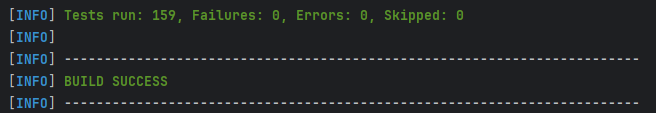
\includegraphics[width=0.8\linewidth]{./obrazy/tests.png}
    %%\caption{Testy}
    %%\label{fig:Testy}
%%\end{figure}

\section{Testy integracyjne}
Testy integracyjne planowane w przyszłości obejmą:
\begin{itemize}
    \item Weryfikację poprawności współpracy między modułami backendowymi.
    \item Sprawdzenie integracji z zewnętrznymi API, takimi jak Alchemy dla Ethereum i Solany.
    \item Testowanie interakcji z bazą danych, w tym poprawności zapisywania i odczytywania danych blockchainowych.
\end{itemize}
